\chapterframe{Linux kernel introduction}

\subchapterframe
{Embedded Linux usage}
{Kernel overview\\
\normalsize Linux features}

\begin{frame}
  \frametitle{Linux kernel in the system}
  \begin{center}
    \includegraphics[width=\textwidth]{slides/sysdev-linux-kernel-intro/linux-kernel-in-system.pdf}
  \end{center}
\end{frame}

\begin{frame}
  \frametitle{History}
  \begin{itemize}
  \item The Linux kernel is one component of a system, which also
    requires libraries and applications to provide features to end
    users.
  \item The Linux kernel was created as a hobby in 1991 by a Finnish
    student, Linus Torvalds.
    \begin{itemize}
    \item Linux quickly started to be used as the kernel for free
      software operating systems
    \end{itemize}
  \item Linus Torvalds has been able to create a large and dynamic
    developer and user community around Linux.
  \item Nowadays, hundreds of people contribute to each kernel
    release, individuals or companies big and small.
  \end{itemize}
\end{frame}

\begin{frame}
  \frametitle{Linux license}
  \begin{itemize}
  \item The whole Linux sources are Free Software released under the
    GNU General Public License version 2 (GPL v2).
  \item For the Linux kernel, this basically implies that:
    \begin{itemize}
    \item When you receive or buy a device with Linux on it, you
      should receive the Linux sources, with the right to study,
      modify and redistribute them.
    \item When you produce Linux based devices, you must release the
      sources to the recipient, with the same rights, with no
      restriction..
    \end{itemize}
  \end{itemize}
\end{frame}

\begin{frame}
  \frametitle{Linux kernel key features}
  \begin{columns}
    \column{0.5\textwidth}
    \begin{itemize}
    \item Portability and hardware support. Runs on most
      architectures.
    \item Scalability. Can run on super computers as well as on tiny
      devices (4 MB of RAM is enough).
    \item Compliance to standards and interoperability.
    \item Exhaustive networking support.
    \end{itemize}
    \column{0.5\textwidth}
    \begin{itemize}
    \item Security. It can't hide its flaws. Its code is reviewed by
      many experts.
    \item Stability and reliability.
    \item Modularity. Can include only what a system needs even at run
      time.
    \item Easy to program. You can learn from existing code. Many
      useful resources on the net.
    \end{itemize}
  \end{columns}
\end{frame}

\begin{frame}
  \frametitle{Supported hardware architectures}
  3.0 status
  \begin{itemize}
  \item See the \code{arch/} directory in the kernel sources
  \item Minimum: 32 bit processors, with or without MMU, and
    \code{gcc} support
  \item 32 bit architectures (\code{arch/} subdirectories)\\
    \code{arm, avr32, blackfin, cris, frv, h8300, m32r, m68k, microblaze, mips, mn10300, parisc, s390, score, sparc, um, unicore32, xtensa}
  \item 64 bit architectures:\\
    \code{alpha, ia64, sparc64, tile}
  \item 32/64 bit architectures\\
    \code{powerpc, x86, sh}
  \item Find details in kernel sources: \code{arch/<arch>/Kconfig},
    \code{arch/<arch>/README}, or \code{Documentation/<arch>/}
  \end{itemize}
\end{frame}

\begin{frame}
  \frametitle{System calls}
  \begin{itemize}
  \item The main interface between the kernel and userspace is the set
    of system calls
  \item About ~300 system calls that provide the main kernel services
    \begin{itemize}
    \item File and device operations, networking operations,
      inter-process communication, process management, memory mapping,
      timers, threads, synchronization primitives, etc.
    \end{itemize}
  \item This interface is stable over time: only new system calls can
    be added by the kernel developers
  \item This system call interface is wrapped by the C library, and
    userspace applications usually never make a system call directly
    but rather use the corresponding C library function
  \end{itemize}
\end{frame}

\begin{frame}
  \frametitle{Virtual filesystems}
  \begin{itemize}
  \item Linux makes system and kernel information available in
    user-space through virtual filesystems.
  \item Virtual filesystems allow applications to see directories and
    files that do not exist on any real storage: they are created on the
    fly by the kernel
  \item The two most important virtual filesystems are
    \begin{itemize}
    \item \code{proc}, for process-related information
    \item \code{sysfs}, for device-related information
    \end{itemize}
  \end{itemize}
\end{frame}

\subchapterframe
{Embedded Linux usage}
{Kernel overview\\
\normalsize Linux versioning scheme and development process}

\begin{frame}
  \frametitle{Until 2.6 (1)}
  \begin{itemize}
  \item One stable major branch every 2 or 3 years
    \begin{itemize}
    \item Identified by an even middle number
    \item Examples: \code{1.0.x, 2.0.x, 2.2.x, 2.4.x}
    \end{itemize}
  \item One development branch to integrate new functionalities and
    major changes
    \begin{itemize}
    \item Identified by an odd middle number
    \item Examples: \code{2.1.x, 2.3.x, 2.5.x}
    \item After some time, a development version becomes the new base
      version for the stable branch
    \end{itemize}
  \item Minor releases once in while: \code{2.2.23, 2.5.12}, etc.
  \end{itemize}
\end{frame}

\begin{frame}
  \frametitle{Until 2.6 (2)}
  \begin{center}
    \includegraphics[width=\textwidth]{slides/sysdev-linux-kernel-intro/old-development-process.pdf}
  \end{center}
\end{frame}

\begin{frame}
  \frametitle{Changes since Linux 2.6 (1)}
  \begin{itemize}
  \item Since \code{2.6.0}, kernel developers have been able to
    introduce lots of new features one by one on a steady pace,
    without having to make major changes in existing subsystems.
  \item So far, there was no need to create a new development branch
    (such as \code{2.7}), which would massively break compatibility
    with the stable branch.
  \item Thanks to this, {\bf more features are released to users at a
      faster pace}.
  \end{itemize}
\end{frame}

\begin{frame}
  \frametitle{Changes since Linux 2.6 (2)}
  Since 2.6.14, the kernel developers agreed on the following
  development model:
  \begin{itemize}
  \item After the release of a \code{2.6.x} version, a two-weeks merge
    window opens, during which major additions are merged.
  \item The merge window is closed by the release of test version
    \code{2.6.(x+1)-rc1}
  \item The bug fixing period opens, for 6 to 10 weeks.
  \item At regular intervals during the bug fixing period,
    \code{2.6.(x+1)-rcY} test versions are released.
  \item When considered sufficiently stable, kernel \code{2.6.(x+1)}
    is released, and the process starts again.
  \end{itemize}
\end{frame}

\begin{frame}
  \frametitle{Merge and bug fixing windows}
  \begin{center}
    \includegraphics[width=\textwidth]{slides/sysdev-linux-kernel-intro/new-development-process.pdf}
  \end{center}
\end{frame}

\begin{frame}
  \frametitle{More stability for the 2.6 kernel tree}
  \begin{columns}
    \column{0.7\textwidth}
    \begin{itemize}
    \item Issue: bug and security fixes only released for most recent
      stable kernel versions.
    \item Some people need to have a recent kernel, but with long term
      support for security updates.
    \item You could get long term support from a commercial embedded
      Linux provider.
    \item You could reuse sources for the kernel used in Ubuntu Long
      Term Support releases (5 years of free security updates).
    \item You could choose one of the versions advertised as “long term”
      in the \url{http://kernel.org} front page. They will be maintained
      longer (2 or 3 years), unlike other versions.
    \end{itemize}
    \column{0.3\textwidth}
    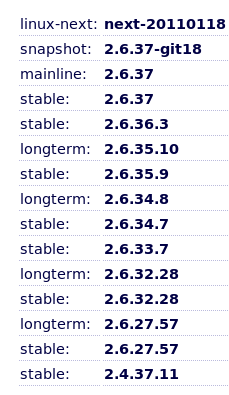
\includegraphics[width=\textwidth]{slides/sysdev-linux-kernel-intro/stable-kernels.png}
  \end{columns}
\end{frame}

\begin{frame}
  \frametitle{New 3.x branch}
  \begin{itemize}
  \item From 2003 to 2011, the official kernel versions were named \code{2.6.x}.
  \item Linux \code{3.0} was released in July 2011
  \item There is no change to the development model, only a change to
    the numbering scheme
    \begin{itemize}
    \item Official kernel versions will be named \code{3.x}
      (\code{3.0, 3.1, 3.2}, etc.)
    \item Stabilized versions will be named \code{3.x.y}
      (\code{3.0.2, 3.4.3}, etc.)
    \item It effectively only removes a digit compared to the previous
      numbering scheme
    \end{itemize}
  \end{itemize}
\end{frame}

\begin{frame}[fragile]
  \frametitle{What's new in each Linux release?}
  \begin{itemize}
  \item The official list of changes for each Linux release is just a
    huge list of individual patches!
\Tiny
    \begin{verbatim}
commit aa6e52a35d388e730f4df0ec2ec48294590cc459
Author: Thomas Petazzoni <thomas.petazzoni@free-electrons.com>
Date:   Wed Jul 13 11:29:17 2011 +0200

    at91: at91-ohci: support overcurrent notification

    Several USB power switches (AIC1526 or MIC2026) have a digital output
    that is used to notify that an overcurrent situation is taking
    place. This digital outputs are typically connected to GPIO inputs of
    the processor and can be used to be notified of those overcurrent
    situations.

    Therefore, we add a new overcurrent_pin[] array in the at91_usbh_data
    structure so that boards can tell the AT91 OHCI driver which pins are
    used for the overcurrent notification, and an overcurrent_supported
    boolean to tell the driver whether overcurrent is supported or not.

    The code has been largely borrowed from ohci-da8xx.c and
    ohci-s3c2410.c.

    Signed-off-by: Thomas Petazzoni <thomas.petazzoni@free-electrons.com>
    Signed-off-by: Nicolas Ferre <nicolas.ferre@atmel.com>
\end{verbatim}
\normalsize
    \begin{itemize}
    \item Very difficult to find out the key changes and to get the
      global picture out of individual changes.
    \end{itemize}
  \item Fortunately, there are some useful resources available
    \begin{itemize}
    \item \url{http://wiki.kernelnewbies.org/LinuxChanges}
    \item \url{http://lwn.net}
    \item \url{http://linuxfr.org}, for French readers
    \end{itemize}
  \end{itemize}
\end{frame}

